% !TEX encoding = UTF-8
% !TEX TS-program = pdflatex
% !TEX root = ../tesi.tex

%**************************************************************
\chapter{Introduzione}
\label{cap:introduzione}
%**************************************************************


% \noindent Esempio di utilizzo di un termine nel glossario \\

% \noindent Esempio di citazione in linea \\
% \cite{site:agile-manifesto}. \\

% \noindent Esempio di citazione nel pie' di pagina \\
% citazione\footcite{womak:lean-thinking} \\
\intro{In questo capitolo viene descritta l'azienda nella quale è stato svolto lo stage e viene spiegato  il progetto di tirocinio.}\\
%**************************************************************
\section{SyncLab}
SyncLab è una Innovative Company collocata in tutta Italia, è nata nel 2002 con sede principale a Napoli ed è cresciuta velocemente. Attualmente, SyncLab ha 6 sedi in tutta italia, più di 300 dipendenti e più di 150 clienti diretti e finali.\\
SyncLab propone servizi innovativi che aiutano i clienti nella realizzazione, progettazione e manutenzione di soluzioni IT.
L'azienda ha collaborato con varie compagnie tra questi i più importanti sono: Tim, Trenitalia, HM, Grimaldi Lines, notartel, sky, eni, enel, vodafone, RayWay, Poste Italiane, Intesa Sanpaolo, Ministero dell'economia delle finanze, fastweb e UniCredit.
\begin{figure}[H]
    \centering
    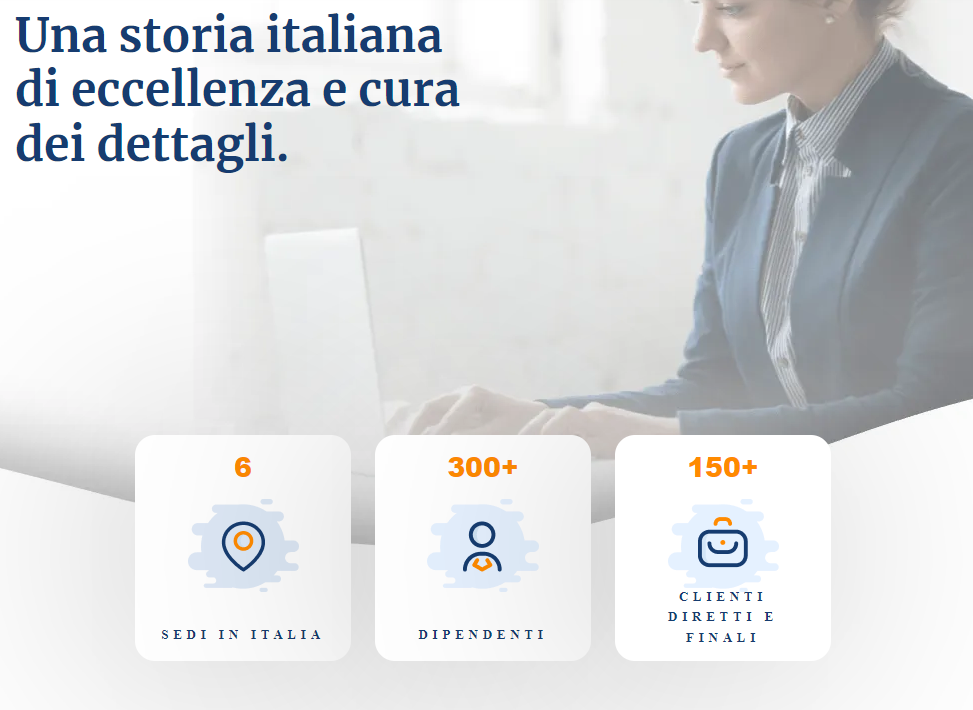
\includegraphics[scale=0.50]{azienda.png}
    \caption{Punti di forza di SyncLab}
\end{figure}
\subsection{Prodotti}
Come accennato, SyncLab opera nel settore IT e i suoi prodotti nascono dalle competenze acquisite e maturate durante i loro 20 anni di collaborazioni. I prodotti coprono vari ambiti come quelli delle telecomunicazioni, utilities, finanza e salute.
\begin{figure}[H]
    \centering
    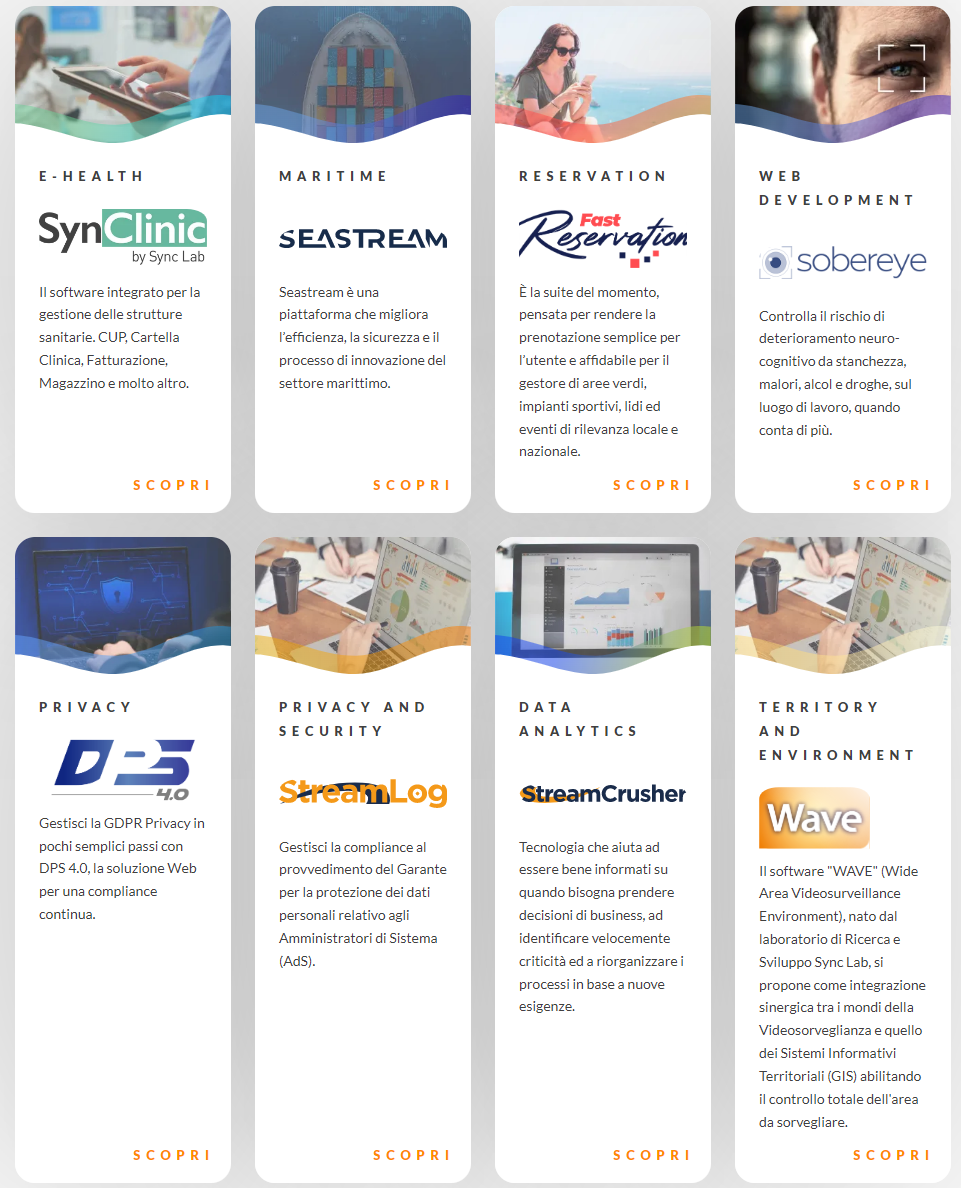
\includegraphics[width=0.55\textwidth]{prodotti.png}
    \caption{I vari prodotti di SyncLab}
\end{figure}
\begin{itemize}
    \item \textbf{SynClinic:} software integrato per la gestione delle strutture sanitarie, il quale offre il sistema di cartella clinica digitale, il servizio di fatturazione, la gestione informatizzata dei farmaci, gli strumenti nativi di gestione amministrativa e tanto altro.
    \item \textbf{SEASTREAM:} una piattaforma nata per migliorare e potenziare le attività di business nel settore armatoriale e di altri operatori del mercato marittimo.
    \item \textbf{FastReservation:} applicazione realizzata per rendere il sistema di prenotazione più facile e affidabile per gli utenti.
    \item \textbf{Sobereye:} soluzione per la sicurezza proattiva per la prevenzione degli incidenti nei settori di trasporti, estrazione, costruzioni e industriale.
    \item \textbf{DPS 4.0:} applicativo che permette di gestire la GDPR Privacy Policy. L'applicativo, tramite una guida semplice sviluppata dagli ingegneri esperti nell'ambito dell'user experience, offre la possibilità di modificare ed aggiornare i documenti sulla privacy con il minimo sforzo.
    \item \textbf{StreamLog:} soluzione per la protezione dei dati personali relativo agli amministratori di sistema, offre la possibilità di effettuare il controllo degli accessi degli utenti ai sistemi in modo semplice ed efficace.
    \item \textbf{StreamCrusher:} tecnologia che serve per aiutare a prendere decisioni di business, indentificando velocemente i punti critici e riformando i processi in base alle nuove esigenze.
    \item \textbf{Wave:} software nato per i sistemi di videosorverglianza, con l'obiettivo di avere una maggiore copertura territoriale col minor numero di telecamere installate e possibilmente utilizzare il minor numero possibile di risorse.
\end{itemize}

\section{Introduzione al progetto}
Lo scopo dello stage quello di realizzare una \gls{webappg} per la gestione delle ordinazioni dei piatti di un ristorante sushi "all you can eat" con tale formula i ristoranti offrono la possibilità di ordinare senza limiti ad un prezzo fisso. Quindi i consumi dei clienti in questi locali è maggiore rispetto ai ristoranti tradizionali, perché con la formula "all-you-can-eat" spesso i clienti mangiano oltre il loro livello di sazietà, in aggiunta a questo il menù contiene centinaia di piatti diversi, il che comporta un elevato numero di ordinazioni da gestire causando così il problema di identificare chi ha ordinato un specifico piatto al momento della consegna.

\section{La soluzione individuata}
SyncLab ha deciso di risolvere questo problema tramite SushiLab, una web-app che offre la possibilità agli utenti di ordinare i piatti e tracciare tutte le ordinazioni. Per semplificare il riconoscimento del piatto nel momento dell'arrivo abbiamo deciso di inserire un'immagine a tutti i piatti.\\ 
Un'utente può inoltre registrarsi alla piattaforma per salvare dei piatti nella propria lista dei preferiti, aggiungere ingredienti alla propria blacklist e recensire un piatto.\\
SushiLab è composta da due parti, la parte \gls{frontendg} e la parte \gls{backendg}. Il back-end deve essere implementato tramite Java utilizzando il framework \gls{Springg} e ha il ruolo pricipale di un web server, che deve comunicare con il data-base, in cui vengono salvate tutte le informazioni dei piatti e tutti gli ordini effettuati dai clienti.
La parte di front-end è invece realizzata in Javascript, utilizzando il framework Angular. La comunicazione tra le due parti della web-app avviene tramite le chiamate \gls{restg} fornite dal back-end.
Ciascuna parte dell'applicazione è stata affidata a più persone. Discutendo con il tutor aziendale, Fabio Pallaro, abbiamo individuato i principali obiettivi per realizzare la web-app ed a me è stato assegnato il compito di sviluppare il front-end dell'applicazione. 
Si è deciso di realizzare una web-app in quanto essa non richiede di scaricare ed installare un'applicativo, così riducendo il tempo delle ordinazioni dei clienti.

\begin{figure}[H]
    \centering
    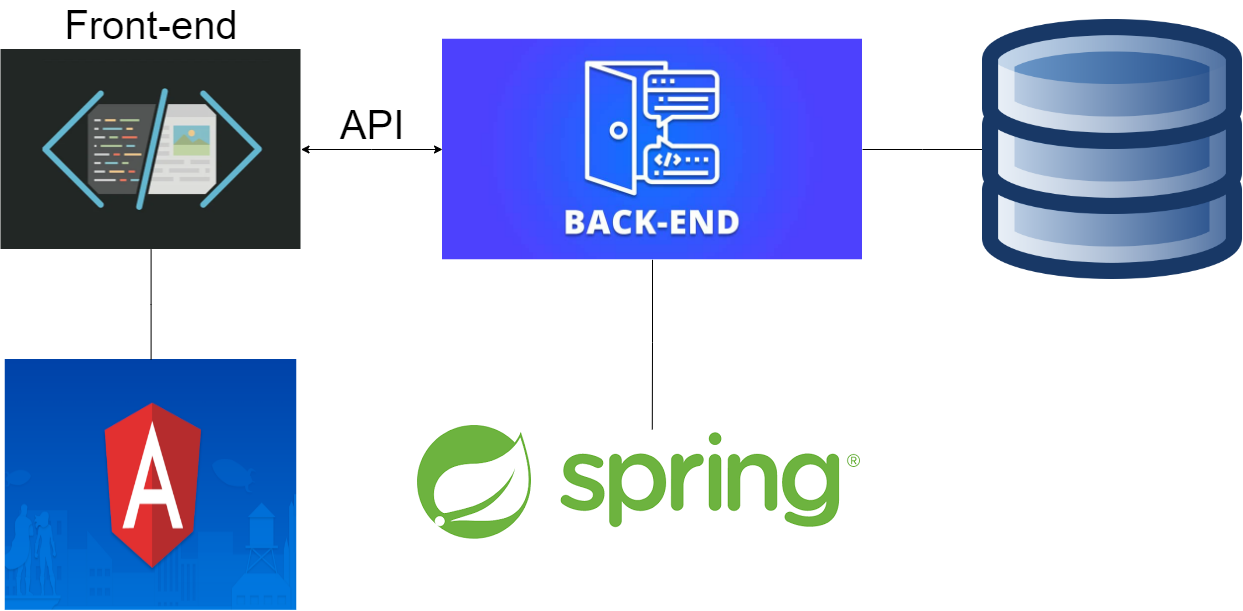
\includegraphics[scale=0.27]{diagramma.png}
    \caption{Diagramma dei componenti della web-app}
\end{figure}
%**************************************************************


%**************************************************************
\section{Organizzazione del testo}

\begin{description}
    \item[{\hyperref[cap:il progetto di stage]{Il secondo capitolo}}] descrive in dettaglio la pianificazione e gli obiettivi dello stage.
    
    \item[{\hyperref[cap:analisi dei requisiti]{Il terzo capitolo}}] descrive i principali casi d'uso e requisiti fondamentali individuati.
    
    \item[{\hyperref[cap:progettazione e codifica]{Il quarto capitolo}}] approfondisce la progettazione e la codifica. La progettazione entra nel dettaglio dell'architettura, delle viste progettate e delle API, mentre la codifica descrive il processo di sviluppo dei principali componenti e service dell'applicazione.
    
    \item[{\hyperref[cap:verifica]{Il quinto capitolo}}] approfondisce la fase di verifica e validazione della web-app.
    
    \item[{\hyperref[cap:conclusioni]{Il sesto capitolo}}] descrive le conclusioni dell'intero progetto, parlando del prodotto finale e le competenze acquisite durante lo stage.
    \item[{\hyperref[cap:appendice a]{A}}] contiene l'elenco completo dei casi d'uso individuati, fornendo una rappresentazione in formato UML e una descrizione formale di essi.
    \item[{\hyperref[cap:appendice b]{B}}] contiene la tabella completa dei requisiti individuati, tracciando ogni requisito alla relativa fonte.
    \item[{\hyperref[cap:appendice c]{C}}] contiene l'elenco completo delle interfacce e dei componenti sviluppati.
\end{description}
Riguardo la stesura del testo, relativamente al documento sono state adottate le seguenti convenzioni tipografiche:
\begin{itemize}
	\item gli acronimi, le abbreviazioni e i termini ambigui o di uso non comune menzionati vengono definiti nel glossario, situato alla fine del presente documento;
	\item per la prima occorrenza dei termini riportati nel glossario viene utilizzata la seguente nomenclatura: \emph{parola}\glsfirstoccur;
	\item i termini in lingua straniera o facenti parti del gergo tecnico sono evidenziati con il carattere \emph{corsivo}.
\end{itemize}